\documentclass[11pt]{article}

\usepackage[margin=1in]{geometry}
\usepackage{booktabs}
\usepackage{array}
\usepackage{longtable}
\usepackage{hyperref}
\usepackage{xcolor}
\usepackage{tikz}
\usepackage{amsmath}
\usepackage{fancyhdr}
\usepackage{caption}
\usepackage{listings}
\usetikzlibrary{arrows.meta,positioning,shapes.geometric,fit,calc}

\hypersetup{
  colorlinks=true,
  linkcolor=blue!60!black,
  urlcolor=blue!60!black,
  citecolor=blue!60!black
}

\pagestyle{fancy}
\setlength{\headheight}{14pt}
\fancyhf{}
\lhead{Obligation-Aware Closure}
\rhead{Nikit Phadke}
\cfoot{\thepage}

\newcommand{\code}[1]{\texttt{\detokenize{#1}}}
\newcommand{\valid}{\textsc{valid}}
\newcommand{\invalid}{\textsc{invalid}}
\newcommand{\unknown}{\textsc{unknown}}
\newcommand{\pass}{\textsc{pass}}
\newcommand{\fail}{\textsc{fail}}
\newcolumntype{L}[1]{>{\raggedright\arraybackslash}p{#1}}
\newcolumntype{C}[1]{>{\centering\arraybackslash}p{#1}}
\setlength{\emergencystretch}{2em}

\lstset{
  basicstyle=\ttfamily\small,
  columns=fullflexible,
  keepspaces=true,
  showstringspaces=false,
  frame=single,
  rulecolor=\color{black!25},
  backgroundcolor=\color{black!2}
}

\title{\textbf{Obligation-Aware Closure:}\\
DLR-O as a Motif Ledger for Terminal Validity}
\author{Nikit Phadke}
\date{June 2026}

\begin{document}
\maketitle

\begin{abstract}
Reliable AI systems fail when they convert local success into global completion
without checking the structural obligations that make a terminal claim valid.
This paper introduces DLR-O, an obligation-ledger layer on top of Disentangled
Language Representation (DLR) and DLR-lambda. DLR provides typed causal and
process representations. DLR-lambda provides recursive recovery from
distributed evidence. DLR-O adds the missing closure semantics: a terminal
claim is \valid{} only when all mandatory motif obligations are satisfied,
\invalid{} when any mandatory blocking obligation is violated, and \unknown{}
when required evidence is unavailable. The central safety property is safe
non-closure: unknown evidence must not be coerced into optimistic success. We
evaluate DLR-O in two synthetic cross-domain experiments spanning graph
traversal, AI agent deletion, compliance approval, payment/order
reconciliation, and code security. In the first experiment, a domain checklist
baseline accepts local terminal claims and fails all five cases, while DLR-O
detects violated obligations and invalidates all false terminal claims. In the
second experiment, an optimistic baseline again fails all five cases by treating
missing evidence as success; DLR-O preserves \unknown{} as a first-class
terminal-validity state and emits safe hold, block, retry, or manual-review
prescriptions. The result supports the thesis that the opposite of
hallucination is not merely accuracy, but obligation-aware closure.
\end{abstract}

\section{Introduction}

Many AI and workflow systems are optimized to produce an answer. That objective
is useful but incomplete. A system can produce the right local answer and still
make an unsafe global claim. A graph traversal can reach the target while part
of the frontier is unavailable. An agent can receive a successful delete result
while backup status is unknown. A compliance system can mark a vendor approved
while sanctions screening has timed out. A payment service can authorize a
charge while capture and order completion remain unreconciled. A web
application can authenticate a user while role scope is unavailable.

These failures share a structure:

\begin{center}
\fbox{\parbox{0.82\linewidth}{
\centering
\textbf{Local Success} $\otimes$ \textbf{Missing Reconciliation}
$\otimes$ \textbf{Unknown Evidence}
$\rightarrow$ \textbf{Terminal Validity Unknown}
}}
\end{center}

The dangerous step is not the local success report itself. It is the coercion
of local success into terminal validity. DLR-O treats local success as an
obligation-generating fact rather than a conclusion. A terminal claim opens a
ledger. The ledger asks which motif obligations must be discharged before the
parent process can close.

This paper freezes the DLR-O result. The central claim is simple:

\begin{quote}
Reliable AI systems require structural obligation ledgers. A terminal claim is
valid only when all mandatory motif obligations are satisfied; invalid when any
mandatory blocking obligation is violated; and unknown when required evidence
is unavailable. Unknown must produce safe non-closure, not optimistic success.
\end{quote}

\section{The DLR Stack}

DLR-O is the terminal-validity layer of a broader stack. Table
\ref{tab:stack} summarizes the roles.

\begin{table}[h]
\centering
\caption{DLR, DLR-lambda, and DLR-O as a reliability stack.}
\label{tab:stack}
\small
\begin{tabular}{L{0.20\linewidth}L{0.31\linewidth}L{0.38\linewidth}}
\toprule
Layer & Function & Failure addressed \\
\midrule
DLR & Structural causal representation & Unstructured summaries that blur local transition, authority, invariant, and terminal outcome. \\
DLR-lambda & Recursive recovery from distributed evidence & Evidence split across traces, chunks, documents, services, or time. \\
DLR-O & Obligation ledger and terminal-validity logic & Premature closure after local success. \\
DLR-O-2 & Unknown-aware closure semantics & Missing evidence coerced into success. \\
\bottomrule
\end{tabular}
\end{table}

DLR is the representational substrate: typed motifs, process status, causal
edges, authority fields, invariants, local/global separation, and terminal
outcomes. DLR-lambda is the recovery procedure: split evidence, recurse over
distributed traces, schedule follow-up retrieval, reconcile contradictions, and
construct ProcessIR. DLR-O is the safety layer. It decides whether a proposed
terminal state is licensed by the obligations generated by the trace.

\section{Motif Obligations}

A motif obligation is a typed requirement generated by a structural fact. For
example, a local terminal claim may generate a terminal-state obligation; an
authority assertion may generate an authority-domain obligation; a destructive
operation may generate a boundary and irreversibility obligation; a distributed
process may generate reconciliation and freshness obligations.

\begin{figure}[h]
\centering
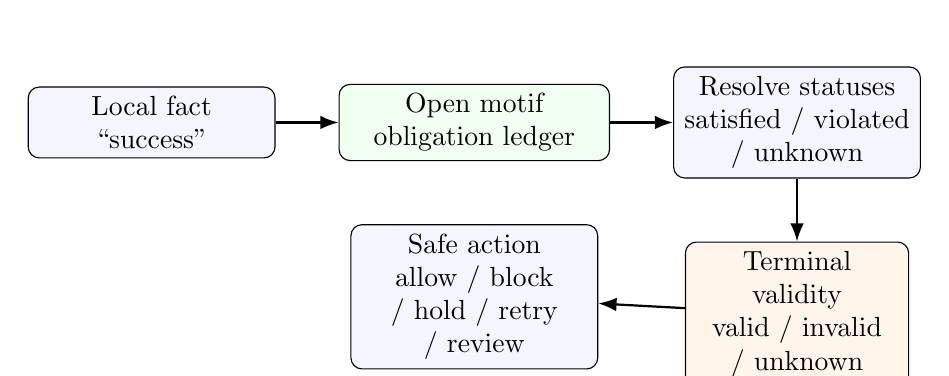
\begin{tikzpicture}[
  node distance=0.8cm,
  box/.style={draw, rounded corners, align=center, minimum height=0.85cm,
    text width=2.9cm, fill=blue!4},
  led/.style={draw, rounded corners, align=center, minimum height=0.85cm,
    text width=3.2cm, fill=green!6},
  terminal/.style={draw, rounded corners, align=center, minimum height=0.85cm,
    text width=2.6cm, fill=orange!8},
  arr/.style={-Latex, thick}
]
\node[box] (fact) {Local fact\\``success''};
\node[led, right=of fact] (ledger) {Open motif\\obligation ledger};
\node[box, right=of ledger] (eval) {Resolve statuses\\satisfied / violated / unknown};
\node[terminal, below=of eval] (term) {Terminal validity\\valid / invalid / unknown};
\node[box, below=of ledger] (safe) {Safe action\\allow / block / hold / retry / review};
\draw[arr] (fact) -- (ledger);
\draw[arr] (ledger) -- (eval);
\draw[arr] (eval) -- (term);
\draw[arr] (term) -- (safe);
\end{tikzpicture}
\caption{DLR-O converts terminal claims into ledgers before allowing closure.}
\label{fig:ledger}
\end{figure}

The important move is that DLR-O does not ask only whether a local action
succeeded. It asks whether the success is licensed at the parent-process level.
This distinction is essential for agent systems and LLM graph traversal, where
tool success is often mistaken for task completion.

\section{Three-Valued Terminal Logic}

DLR-O uses three terminal-validity states:

\begin{itemize}
\item \valid{}: all mandatory blocking obligations are satisfied.
\item \invalid{}: at least one mandatory blocking obligation is violated.
\item \unknown{}: no mandatory blocking obligation is known to be violated, but
at least one required obligation remains unresolved.
\end{itemize}

The rule is intentionally small:

\begin{lstlisting}[caption={Minimal terminal-validity rule.}]
type ObligationStatus = "satisfied" | "violated" | "unknown";
type TerminalValidity = "valid" | "invalid" | "unknown";

function terminalValidity(obligations: Obligation[]): TerminalValidity {
  const mandatory = obligations.filter(o => o.mandatory);
  if (mandatory.some(o => o.status === "violated")) {
    return "invalid";
  }
  if (mandatory.some(o => o.status === "unknown")) {
    return "unknown";
  }
  return "valid";
}
\end{lstlisting}

This rule is not a complete policy engine. A deployment may add severity,
blocking status, and safe defaults:

\begin{lstlisting}[caption={Policy refinements for deployment.}]
type SafeDefault = "allow" | "deny" | "pending" | "manual_review" | "retry";

type Obligation = {
  id: string;
  mandatory: boolean;
  blocking: boolean;
  status: "satisfied" | "violated" | "unknown";
  safeDefault: SafeDefault;
};
\end{lstlisting}

However, the core safety property is independent of domain policy:
unavailable evidence is not success. In privileged, destructive, compliance, or
terminal contexts, \unknown{} should normally block, pend, retry, or escalate.

\section{Experiment 1: Cross-Domain Obligation Transfer}

\subsection{Objective}

The first experiment tests whether motif obligations are substrate-independent
rather than log-specific. The same obligation ledger is applied to graph
traversal, agent deletion, compliance approval, payment/order reconciliation,
and code security.

\subsection{Systems}

\begin{itemize}
\item \textbf{Domain checklist baseline}: accepts the local terminal claim and
emits only a shallow terminal obligation.
\item \textbf{DLR-O cross-domain obligation ledger}: infers motif obligations,
resolves statuses, determines terminal validity, and emits a motif-level
prescription.
\end{itemize}

\subsection{Cases}

\begin{longtable}{L{0.20\linewidth}L{0.24\linewidth}L{0.43\linewidth}}
\caption{DLR-O cross-domain transfer cases.}
\label{tab:o_cases}\\
\toprule
Domain & Local success & Missing or violated obligation \\
\midrule
\endfirsthead
\toprule
Domain & Local success & Missing or violated obligation \\
\midrule
\endhead
Graph traversal & Target reached & Frontier exhaustion and global traversal completion. \\
Agent deletion & Delete tool succeeded & Canonical boundary, authority over target, and rollback evidence. \\
Compliance approval & Vendor approved & Authority domain and sanctions-screening invariant. \\
Payment/order & Payment authorized & Capture, inventory, and order/payment reconciliation. \\
Code security & User authenticated & Role scope, resource boundary, and authorization invariant. \\
\bottomrule
\end{longtable}

\subsection{Results}

\begin{table}[h]
\centering
\caption{Experiment 1 summary.}
\label{tab:o_summary}
\small
\setlength{\tabcolsep}{2pt}
\begin{tabular}{L{0.32\linewidth}C{0.12\linewidth}C{0.16\linewidth}C{0.15\linewidth}C{0.15\linewidth}}
\toprule
System & Pass rate & Obligation recall & Status accuracy & Terminal accuracy \\
\midrule
Domain checklist baseline & 0.0000 & 0.0000 & 0.0000 & 0.0000 \\
DLR-O obligation ledger & 1.0000 & 1.0000 & 1.0000 & 1.0000 \\
\bottomrule
\end{tabular}
\end{table}

\begin{table}[h]
\centering
\caption{Experiment 1 case-level outcomes.}
\label{tab:o_case_scores}
\scriptsize
\setlength{\tabcolsep}{2pt}
\begin{tabular}{L{0.19\linewidth}L{0.14\linewidth}L{0.17\linewidth}C{0.06\linewidth}C{0.08\linewidth}C{0.08\linewidth}C{0.08\linewidth}}
\toprule
Case & Domain & System & Pass & Recall & Status & Terminal \\
\midrule
O1 frontier false terminal & graph traversal & Checklist & \fail & 0.0000 & 0.0000 & no \\
O1 frontier false terminal & graph traversal & DLR-O & \pass & 1.0000 & 1.0000 & yes \\
O2 boundary authority & agent deletion & Checklist & \fail & 0.0000 & 0.0000 & no \\
O2 boundary authority & agent deletion & DLR-O & \pass & 1.0000 & 1.0000 & yes \\
O3 false vendor approval & compliance & Checklist & \fail & 0.0000 & 0.0000 & no \\
O3 false vendor approval & compliance & DLR-O & \pass & 1.0000 & 1.0000 & yes \\
O4 authorized not complete & payment/order & Checklist & \fail & 0.0000 & 0.0000 & no \\
O4 authorized not complete & payment/order & DLR-O & \pass & 1.0000 & 1.0000 & yes \\
O5 authn not authz & code security & Checklist & \fail & 0.0000 & 0.0000 & no \\
O5 authn not authz & code security & DLR-O & \pass & 1.0000 & 1.0000 & yes \\
\bottomrule
\end{tabular}
\end{table}

The result is deliberately not about broad statistical generalization. It is a
controlled falsification of a closure rule. The baseline fails because it treats
the local terminal report as sufficient. \mbox{DLR-O} succeeds because it opens the
right ledger: frontier reconciliation for traversal, boundary and authority for
deletion, sanctions and authority for compliance, capture/reconciliation for
orders, and authorization/resource boundary for code security.

\section{Experiment 2: Unknown-Aware Safe Non-Closure}

\subsection{Objective}

The second experiment stress-tests the most important reliability condition:
terminal validity must remain \unknown{} when mandatory evidence is
unavailable. Unknown is not a failure to answer. It is a valid
terminal-validity state.

\subsection{Systems}

\begin{itemize}
\item \textbf{Optimistic terminal baseline}: accepts the local success claim as
\valid{}.
\item \textbf{DLR-O unknown-aware ledger}: opens obligations and preserves
\unknown{} when required evidence is unavailable.
\end{itemize}

\subsection{Cases}

\begin{table}[h]
\centering
\caption{DLR-O-2 unknown-handling cases.}
\label{tab:unknown_cases}
\small
\begin{tabular}{L{0.20\linewidth}L{0.24\linewidth}L{0.43\linewidth}}
\toprule
Domain & Local success & Unknown evidence \\
\midrule
Graph traversal & Target reached & One shard unavailable; frontier completeness unknown. \\
Agent deletion & Delete tool succeeded & Backup or rollback status unknown. \\
Compliance approval & Vendor approved & Sanctions provider timed out. \\
Payment/order & Payment authorized & Capture status unavailable. \\
Code security & User authenticated & Role service unavailable. \\
\bottomrule
\end{tabular}
\end{table}

\subsection{Results}

\begin{table}[h]
\centering
\caption{Experiment 2 summary.}
\label{tab:unknown_summary}
\small
\setlength{\tabcolsep}{2pt}
\begin{tabular}{L{0.32\linewidth}C{0.12\linewidth}C{0.14\linewidth}C{0.18\linewidth}C{0.14\linewidth}}
\toprule
System & Pass rate & Unknown recall & Overconfident success & Terminal accuracy \\
\midrule
Optimistic terminal baseline & 0.0000 & 0.0000 & 1.0000 & 0.0000 \\
DLR-O unknown-aware ledger & 1.0000 & 1.0000 & 0.0000 & 1.0000 \\
\bottomrule
\end{tabular}
\end{table}

\begin{table}[h]
\centering
\caption{Experiment 2 case-level outcomes.}
\label{tab:unknown_scores}
\scriptsize
\setlength{\tabcolsep}{2pt}
\begin{tabular}{L{0.19\linewidth}L{0.14\linewidth}L{0.17\linewidth}C{0.06\linewidth}C{0.10\linewidth}C{0.07\linewidth}C{0.09\linewidth}}
\toprule
Case & Domain & System & Pass & Unknown recall & Terminal & Overconf. \\
\midrule
S1 unavailable subgraph & graph traversal & Optimistic & \fail & 0.0000 & no & yes \\
S1 unavailable subgraph & graph traversal & DLR-O & \pass & 1.0000 & yes & no \\
S2 backup unknown & agent deletion & Optimistic & \fail & 0.0000 & no & yes \\
S2 backup unknown & agent deletion & DLR-O & \pass & 1.0000 & yes & no \\
S3 provider timeout & compliance & Optimistic & \fail & 0.0000 & no & yes \\
S3 provider timeout & compliance & DLR-O & \pass & 1.0000 & yes & no \\
S4 capture unavailable & payment/order & Optimistic & \fail & 0.0000 & no & yes \\
S4 capture unavailable & payment/order & DLR-O & \pass & 1.0000 & yes & no \\
S5 role service unavailable & code security & Optimistic & \fail & 0.0000 & no & yes \\
S5 role service unavailable & code security & DLR-O & \pass & 1.0000 & yes & no \\
\bottomrule
\end{tabular}
\end{table}

Across all five domains, the optimistic baseline makes the same mistake:
\[
\text{local success} \rightarrow \text{terminal valid}.
\]
DLR-O instead applies:
\[
\text{local success} \rightarrow \text{open obligations}
\rightarrow \text{missing evidence} \rightarrow \text{terminal unknown}.
\]
The prescription is safe non-closure: hold, block, retry, or manual review.

\section{Discussion}

\subsection{Why Unknown Matters}

Binary terminal logic forces unsafe closure. A system must either approve or
reject, finish or fail, allow or forbid. Real systems often need a third state:
not enough evidence to close. DLR-O makes this state explicit. This matters
most in terminal contexts, where a premature \valid{} decision can trigger
irreversible action, privileged access, compliance exposure, or downstream
automation.

\subsection{From Hallucination to Closure}

The usual framing of AI reliability centers on factual accuracy. Accuracy is
necessary but not sufficient. The deeper failure in the evaluated cases is an
unauthorized terminal transition. The system is not merely wrong; it closes a
process it was not licensed to close. In that sense, the opposite of
hallucination is not only accuracy. The opposite of hallucination is
obligation-aware closure.

\subsection{Transfer Across Domains}

DLR-O transfers because it does not depend on domain nouns. It depends on
structural questions:

\begin{itemize}
\item Was the authority valid for this transition and boundary?
\item Were mandatory invariants preserved?
\item Was local success reconciled with parent-process completion?
\item Was evidence fresh and complete at the time of the terminal claim?
\item If evidence is unavailable, what safe default is required?
\end{itemize}

The same questions apply to graph traversal, agent tools, compliance workflows,
orders, and security checks. This is the practical value of motif-level
representation: it gives the system a reusable grammar for closure.

\section{Limitations}

The experiments are synthetic and deterministic. They are designed to isolate
closure semantics rather than measure natural-language extraction performance
on a broad benchmark. The baselines are intentionally simple, because the
claim under test is structural: accepting local success as terminal validity is
unsafe. Future work should compare against LLM agents, workflow orchestrators,
security policy engines, and graph-reasoning systems on larger natural traces.

The current rule also treats mandatory violated obligations as dominant over
unknown obligations. In real deployments, evidence may conflict rather than
merely disappear. A natural DLR-O-3 extension would add conflict obligations
and ledger revision. Examples include one shard asserting an edge while
another reports deletion, one sanctions provider clearing a vendor while
another flags it, or a payment processor reporting capture while the ledger
remains unsettled.

\section{Conclusion}

DLR-O completes the reliability endpoint of the DLR stack. DLR represents
process structure. DLR-lambda recovers that structure from distributed
evidence. DLR-O decides whether a terminal claim is licensed by the mandatory
obligations generated by the process.

The completed terminal logic is:
\[
\begin{aligned}
\text{satisfied mandatory obligations} &\rightarrow \valid{} \\
\text{violated mandatory blocking obligation} &\rightarrow \invalid{} \\
\text{unknown mandatory blocking obligation} &\rightarrow \unknown{}
\end{aligned}
\]

This is the reliability primitive: a system is not reliable because it always
answers. It is reliable because it knows when it is not allowed to close.

\appendix

\section{Reproduction Commands}

The experiments can be regenerated with:

\begin{lstlisting}
npm run run:dlr-o
npm run run:dlr-o-stress
\end{lstlisting}

The generated reports are:

\begin{itemize}
\item \code{dlr_obligation_transfer.md}
\item \code{artifacts/dlr_obligation_transfer.json}
\item \code{dlr_obligation_stress.md}
\item \code{artifacts/dlr_obligation_stress.json}
\end{itemize}

\begin{thebibliography}{9}

\bibitem{dlr_lambda_1}
Nikit Phadke.
\newblock \emph{Recursive Log Diagnosis with ProcessIR: A DLR-Lambda
Experiment on Loghub}.
\newblock 2026.

\bibitem{dlr_lambda_2}
Nikit Phadke.
\newblock \emph{From Batch Reduction to Investigative Fixpoint: A
DLR-Lambda-2 Experiment on Marker-Free Log Diagnosis}.
\newblock 2026.

\bibitem{dlr_lambda_3}
Nikit Phadke.
\newblock \emph{DLR-Lambda-3 Motif Obligation Calculus}.
\newblock 2026.

\bibitem{processir}
Nikit Phadke.
\newblock \emph{Trace-to-Causal-IR Diagnosis and Hidden Preconditions}.
\newblock 2026.

\end{thebibliography}

\end{document}
